\appendix
\chapter{Anhang}
Appendix
\section{Graph-Datenbanken - Grundlegende technologische Aspekte}
\section{Graph-Datenbanken und -Frameworks - Ausgewählte Systeme}
\begin{figure}[H]

    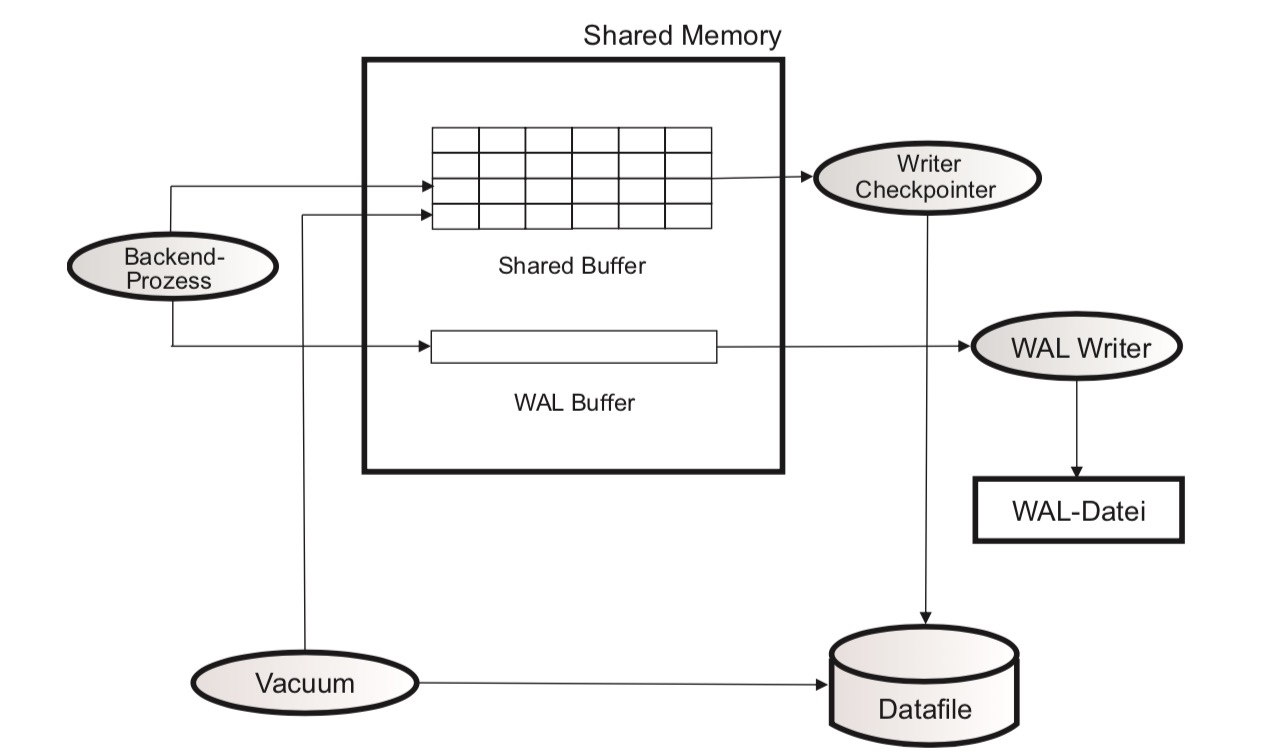
\includegraphics[width = \linewidth]{images/postgresArchitektur.jpg}
    \caption{Postgres Architektur}
    \label{Postgres Architektur}

\end{figure}
\section{Graph-Datenbanken im praktischen Einsatz: OLTP}
\begin{lstlisting}[language=SQL,caption=CSV Input,frame=single]
    \copy Beitraege
    FROM './data/Beitraege.csv' DELIMITER ',' CSV HEADER;
\end{lstlisting}


\begin{lstlisting}[language=SQL,caption=Anlegen der Tabelle facebook-profiles,frame=single]
    CREATE TABLE public."facebook-profiles"
    (
    id serial PRIMARY KEY,
    first TEXT,
    last TEXT,
    gender TEXT,
    country TEXT,
    birth TEXT
    );
\end{lstlisting}

\begin{lstlisting}[language=SQL,caption=Anlegen der Tabelle facebook,frame=single]
    CREATE TABLE public.facebook
    (
    src INT,
    dst INT,
    type TEXT,
    date TEXT
    );
\end{lstlisting}

\begin{lstlisting}[language=SQL,caption=Hinzufügen von Fremdschlüsseln,frame=single]
    ALTER TABLE public.facebook
    ADD CONSTRAINT "facebook_facebook-profiles_id_fk"
    FOREIGN KEY (src) REFERENCES public."facebook-profiles" (id)
\end{lstlisting}

\section{Graph-Datenbanken im praktischen Einsatz: OLAP}
%\chapter{Anhang}
%Appendix